\documentclass[9pt,xcolor=svgnames,aspectratio=169]{beamer}

\usepackage{packages}

\title{Introduction to Lattice Quantum Gravity}
\author[Name]{Timo Jakobs}
%\subtitle{Subtitle}
\institute[uni]{Bethe Center for Theoretical Physics \\ University of Bonn}
\date{\today}
%\titlegraphic{\vspace{-0.5cm}\hfill\includegraphics[scale=0.23]{logo.png}}


\begin{document}
{
\setbeamercolor{background canvas}{bg=NavyBlue!50!DarkOliveGreen, fg=white}
\setbeamercolor{normal text}{fg=white}
\maketitle
}%This is the colour of the first slide. bg= background and fg=foreground
\metroset{titleformat frame=smallcaps}
%
% \begin{frame}{Outline}
%  \setbeamertemplate{section in toc}[sections numbered]
%  \tableofcontents[hideallsubsections]
% \end{frame}

% \section{TODO}
%
% \begin{frame}{TODO}
%   \begin{itemize}
%     \item Ziele Grenzwerte der Monte Carlo
%     \item Phasendiagram am Anfang
%   \end{itemize}
% \end{frame}
%
% \begin{frame}{TODO - Questions}
%   \begin{itemize}
%     \item Check and Add Sources
%     \item Explain what a Simplex is
%   \end{itemize}
% \end{frame}
\section{What the heck is quantum gravity anyway?}


\begin{frame}{What the heck is quantum gravity anyway?}
 \begin{columns}[onlytextwidth,t]
  \uncover<1->{\begin{column}{0.48\textwidth}
    \begin{block}{Classical Gravity}
     \vspace{0pt}
     Einstein Field equations:
     \begin{align*}
      \uncoverubrace<2->{\frac{8 \pi G}{c^4}}{\kappa}\uncoverubrace<2->{T_{\mu\nu}}{\substack{\text{stuff within} \\  \text{space-time}}} & = \uncoverubrace<2->{R_{\mu\nu} - \frac{1}{2} R g_{\mu\nu} + \Lambda g_{\mu \nu}}{\text{geometry of space-time}}
      \uncover<3->{\intertext{Einstein Hilbert Action (for $T_{\mu\nu} = 0$):}
      S_{EH} [g] & = -\frac{1}{2 \kappa} \int \mathrm{d}^4 x \sqrt{-\mathrm{det} \, g} \, (R - 2\Lambda)}
     \end{align*}
    \end{block}
   \end{column}}
  \begin{column}{0.48\textwidth}
   \uncover<4->{\begin{block}{Quantum Gravity}
     \vspace{0pt}
     Path integral formulation:
     \begin{align*}
      Z_E & = \int \mathcal{D} g \, \exp \left( - S[g]\right)
     \end{align*}
    \end{block}}
   \uncover<5->{\textbf{Problems}
    \begin{itemize}
     \item non renormalizable coupling expansion
     \item might still be asymptotically safe \\ $\Rightarrow$ non-pertubative approaches
    \end{itemize}}
  \end{column}
 \end{columns}
\end{frame}


\section{Regge Action}


\begin{frame}{Simplical Gravity}
 \begin{columns}
  \begin{column}{0.52\textwidth}
   \begin{block}{Simplical Gravity - Regge Action}
    \vspace{0pt}
    \begin{itemize}
     \item Geometry described by:\\
           $\qquad$ metric $g_{\mu\nu}$ $\rightarrow$ triangulation $T$
           \uncover<2->{\item Regge Action:
           \begin{align*}
            S_{\textrm{R}} & = - \kappa \sum_{i=1}^{N_2} \mathrm{Vol}(\sigma_i^2) \varepsilon_i + \kappa \Lambda \sum_{i=1}^{N_4} \mathrm{Vol}(\sigma_i^4)     \intertext{where}
            N_j            & \equiv \#j\text{-simplices}                                                                                                                         \\
            \varepsilon_i  & \equiv \text{deficit angle at hinge}\,\, i                                                                                                          \\
            \sigma_i^j     & \equiv i\text{th}\,\, j\text{-Simplex}
           \end{align*}}
    \end{itemize}
   \end{block}
  \end{column}
  \begin{column}{0.46\textwidth}
   \begin{figure}
    \centering
    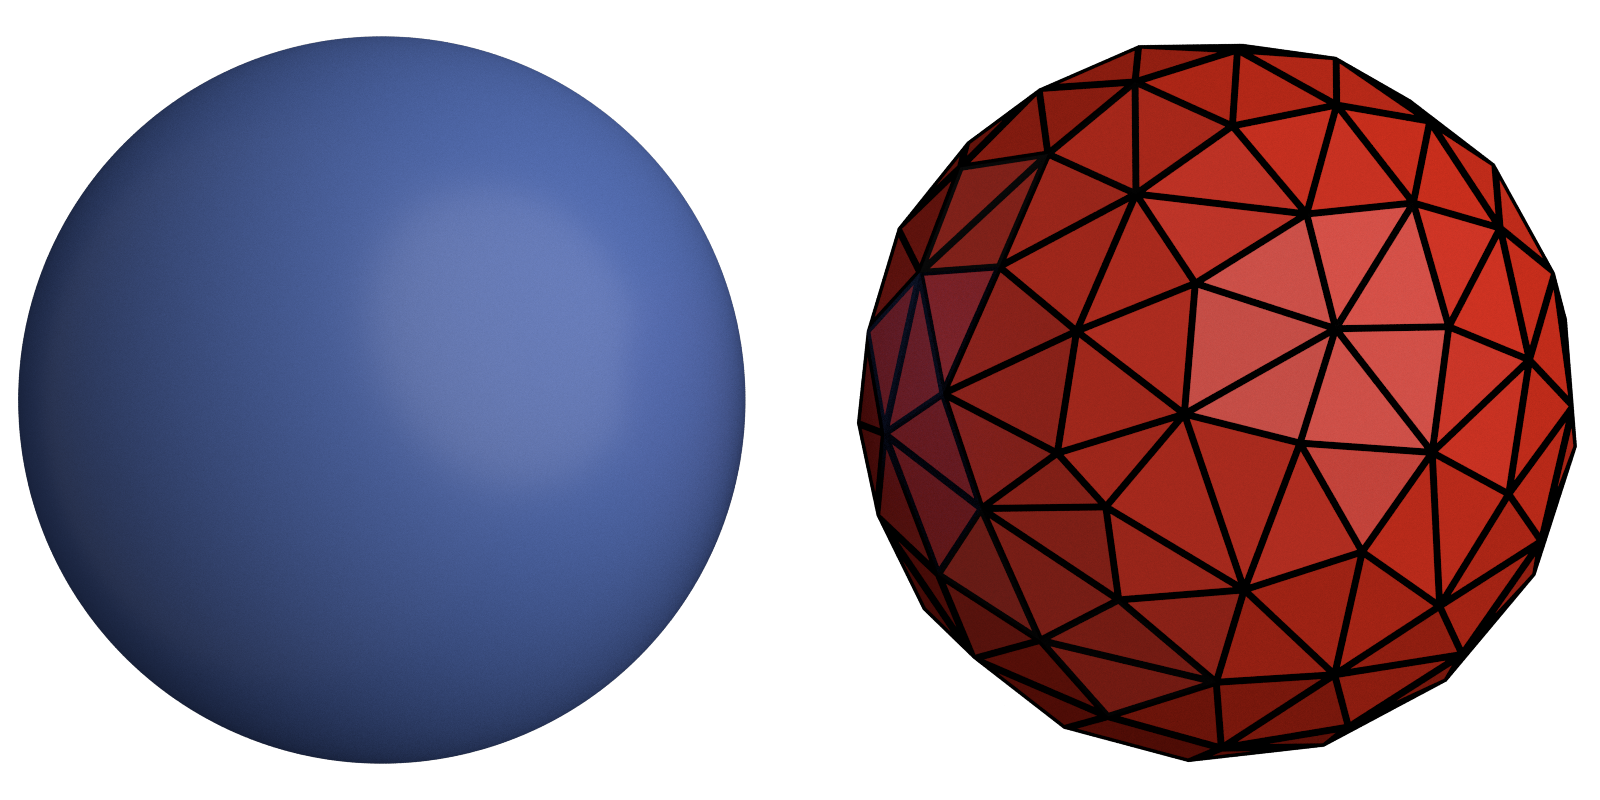
\includegraphics[width=0.9\textwidth]{pics/triangulation-fib.png}
   \end{figure}
   \only<1-3>{\uncover<3>{\begin{block}{2D}
     \vspace{-0.5cm}
     \centering
     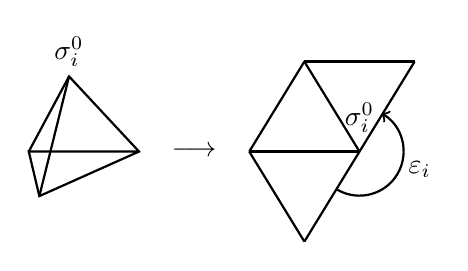
\begin{tikzpicture}[scale=1]
 \def\a{1.40}
 \def\b{0.5}
 \def\trigConst{0.816497}

 \begin{scope} [x     = {(1cm,0)},
   y     = {({0.7cm*cos(135)},{-0.7cm*sin(135)})},
   z     = {(0,1cm)}]


  \path coordinate (T1) at ({-(0.5*\a)}, {0.3333*\trigConst*\a}, {\trigConst*\a})
  coordinate (A1) at (0,0,0)
  coordinate (B1) at ({-\a},0,0)
  coordinate (C1) at ({-(0.5*\a)},{\trigConst*\a},0)
  coordinate (E1) at ({-(0.5*\a)}, {0.3333*\trigConst*\a}, {-\trigConst*\a});

  \draw[thick]  (A1) -- (B1) -- (C1) -- (A1) -- (T1) -- (B1);
  \draw[thick]  (T1) -- (C1);
  \node(h1)[anchor=south] at (T1) {$\sigma^0_i$};

 \end{scope}
 \node[align=center] at (0.5 * \a,0) {$\longrightarrow$};
 \begin{scope} [x     = {(1cm,0)},
   y     = {(0,1cm)},shift={(2*\a,0)}]

  %1st Triangle
  \draw[thick] (-\a,0) -- (0, 0);
  \draw[thick] (-\a,0) -- ({-(0.5*\a)}, {\trigConst * \a});
  \draw[thick] (0,0)  -- ({-(0.5*\a)}, {\trigConst * \a});

  %2nd Triangle
  \draw[thick] (-\a,0) -- ({-(0.5*\a)}, -{\trigConst * \a});
  \draw[thick] (0,0)    -- ({-(0.5*\a)}, -{\trigConst * \a});

  \draw[thick] (-0.5*\a, \trigConst * \a) -- (-0.5*\a + \a, \trigConst * \a);
  \draw[thick] (0,0) -- (-0.5*\a + \a, \trigConst * \a);
  \draw[thick,->] ([shift=(-120:0.4*\a)]0,0) arc (-120:60:0.4*\a);

  \node(h2)[anchor=south] at (0,0.12cm) {$\sigma^0_i$};
  \node(h3)[anchor=north west] at (0.5cm,0) {$\varepsilon_i$};

 \end{scope}
\end{tikzpicture}

    \end{block}}}
   \only<4>{\begin{block}{3D}
     \vspace{-0.5cm}
     \centering
     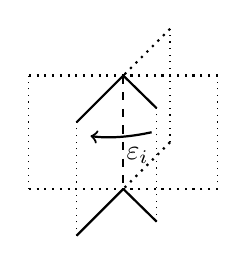
\begin{tikzpicture}[scale=1]
 \def\a{1.2}

 \begin{scope} [x     = {(1cm,0)},
   y     = {({0.7cm*cos(135)},{-0.7cm*sin(135)})},
   z     = {(0,1cm)}]


  \path coordinate (CB) at (0,0,0)
  coordinate (CT) at (0,0,1.2*\a)
  coordinate (AB) at (0.7*\a,0.7*\a,0)
  coordinate (AT) at (0.7*\a,0.7*\a,1.2*\a)
  coordinate (BB) at (0,\a,0)
  coordinate (BT) at (0,\a,1.2*\a)
  coordinate (DB) at (\a,0,0)
  coordinate (DT) at (\a,0,1.2*\a)
  coordinate (FB) at (-\a,0,0)
  coordinate (FT) at (-\a,0,1.2*\a)
  coordinate (EB) at (0,-\a,0)
  coordinate (ET) at (0,-\a,1.2*\a);


  \draw[thick, dashed]  (CT) -- (CB);

  \draw[thick]  (AT) -- (CT);
  \draw[thick]  (AB) -- (CB);
  \draw[dotted] (AB) -- (AT);

  \draw[thick]  (BT) -- (CT);
  \draw[thick]  (BB) -- (CB);
  \draw[dotted] (BB) -- (BT);

  \draw[thick,dotted]  (DT) -- (CT);
  \draw[thick,dotted]  (DB) -- (CB);
  \draw[dotted] (DB) -- (DT);

  \draw[thick,dotted]  (ET) -- (CT);
  \draw[thick,dotted]  (EB) -- (CB);
  \draw[dotted] (EB) -- (ET);

  \draw[thick,dotted]  (FT) -- (CT);
  \draw[thick,dotted]  (FB) -- (CB);
  \draw[dotted] (FB) -- (FT);

  \draw[thick,->] (0.3*\a,0,0.6*\a) arc [start angle=60,end angle=105, radius=0.8*\a,y radius=0.8*\a];

  \node(e)[] at (0.3*\a,0.3*\a,0.5*\a) {$\varepsilon_i$};

 \end{scope}

\end{tikzpicture}

    \end{block}}
  \end{column}
 \end{columns}
\end{frame}

\begin{frame}{Simplical Gravity}
 \begin{columns}
  \begin{column}{0.52\textwidth}
   \begin{block}{Further Restrictions}
    \vspace{0pt}
    \begin{itemize}
     \item Restriction to equilateral simplices with side length $a$
     \item Lattice action:\begin{align*}
            S_{ER} = - \kappa_2(\kappa,a) N_2 + \kappa_4(\kappa,\Lambda, a) N_4 + \lambda\abs{N_4 - V}
           \end{align*}
     \item Triangulations only differ by number and configuration of simplices
    \end{itemize}
    \begin{block}{Partition Function:}
     \vspace{0pt}
     \begin{align*}
      Z_E = \sum_{\boldsymbol{T}} \frac{1}{C_T} \mathrm{e}^{-S_{ER}}
     \end{align*}
    \end{block}
   \end{block}
  \end{column}
  \begin{column}{0.46\textwidth}
   \begin{figure}
    \centering
    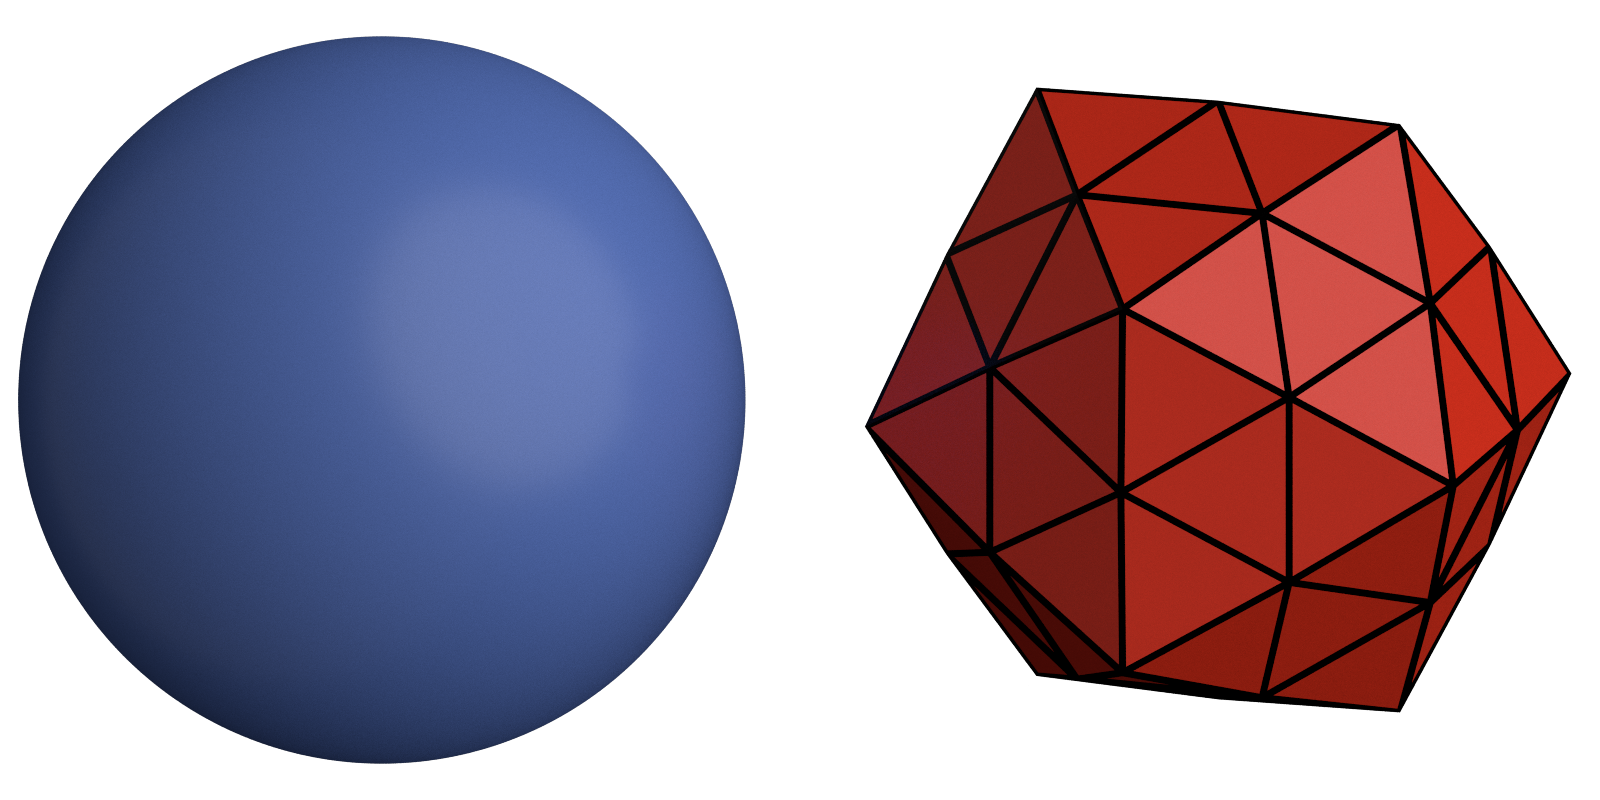
\includegraphics[width=0.9\textwidth]{pics/triangulation-ico.png}
    \caption{\tiny{rendered with the fresnel library (\url{https://github.com/glotzerlab/fresnel})}}
   \end{figure}
  \end{column}
 \end{columns}
\end{frame}

\begin{frame}{Metropolis Monte Carlo Methods}
 \begin{columns}
  \begin{column}{0.46\textwidth}
   \uncover<1->{\vspace{0.5cm}\\Used to solve path integrals numerically:
    \begin{align*}
     \left\langle \mathcal{O} \right\rangle & = \frac{1}{Z}\sum_{\boldsymbol{T}} \frac{1}{C_T} \, \mathcal{O} \exp \left( - S(\boldsymbol{T})\right)
    \end{align*}}
   \uncover<2->{$\left\langle \mathcal{O} \right\rangle$  approximated by generating random  configuration $\boldsymbol{T}$ with distribution
    \begin{align*}
     \rho (\boldsymbol{T})                  & = \frac{1}{Z} \exp \left( - S(\boldsymbol{U})\right) \intertext{and thus}
     \left\langle \mathcal{O} \right\rangle & = \frac{1}{\#\{ \boldsymbol{T}\}} \sum_{\boldsymbol{T} \in \{ \boldsymbol{T}\}} \mathcal{O}(\boldsymbol{T})
    \end{align*}}
  \end{column}
  \begin{column}{0.52\textwidth}
   \begin{algorithmic}[1]
    \uncover<3->{\STATE {$\boldsymbol{T}\leftarrow$ (\text{initial configuration})}}
    \uncover<4->{\FOR {$N$ iterations}}
    \uncover<5->{\STATE {$\boldsymbol{T}' \leftarrow \text{update}(\boldsymbol{T})$}}
    \uncover<6->{\STATE {$\Delta S \leftarrow S(\boldsymbol{T}) - S(\boldsymbol{T}')$}}
    \uncover<7->{\IF {$\Delta S < 0 \, \text{or} \, \exp \left(- \Delta S \right) > \text{rand}(0,1)$}}
    \uncover<7->{\STATE $\boldsymbol{T} \leftarrow \boldsymbol{T}'$}
    \uncover<7->{\ENDIF}
    \uncover<8->{\STATE measure observables}
    \uncover<4->{\ENDFOR}
   \end{algorithmic}
  \end{column}
 \end{columns}
\end{frame}

\begin{frame}{Pachner Moves}
 %Local Update Moves for Metropolis-Monte-Carlo simulations:
 \begin{columns}[onlytextwidth,t]
  \begin{column}{0.37\textwidth}
   \uncover<1->{\begin{block}{Requirements for updates}
     \vspace{0pt}
     \begin{itemize}
      \uncover<2->{\item maintain topology}
            \uncover<3->{\item relate all triangulations with same topology}
     \end{itemize}
     \uncover<4->{$\qquad\longrightarrow$ Ergodicity}
    \end{block}}
   \vspace{0.5cm}
   \uncover<8->{\begin{block}{4D}
     \vspace{0pt}
     \begin{itemize}
      \item 5 Pachner moves in 4D:\\
            $(1,5)$,$(2,4)$,$(3,3)$,$(4,2)$,$(5,1)$
     \end{itemize}
    \end{block}}
  \end{column}
  \uncover<5->{\begin{column}{0.34\textwidth}
    \begin{block}{2D}
     \vspace{0pt}
     \uncover<5->{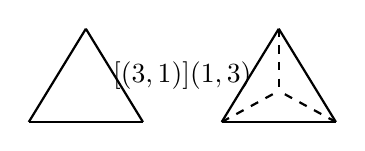
\begin{tikzpicture}
 \def\a{1.45}
 \def\b{0.5}
 \def\trigConst{0.816497}

 %1st Triangle
 \draw[thick] (-\a-\b,0) -- (-\b, 0);
 \draw[thick] (-\a-\b,0) -- ({-\b-(0.5*\a)}, {\trigConst * \a});
 \draw[thick] (-\b,0)    -- ({-\b-(0.5*\a)}, {\trigConst * \a});

 %2nd Triangle
 \draw[thick] (\a + \b,0) -- (\b, 0);
 \draw[thick] (\a+\b,0)   -- ({\b+(0.5*\a)}, {\trigConst * \a});
 \draw[thick] (\b,0)      -- ({\b+(0.5*\a)}, {\trigConst * \a});

 %Lines to center
 \draw[thick, dashed] (\b,0)                             -- ({\b+(0.5*\a)}, {\trigConst * \a * 0.33333});
 \draw[thick, dashed] (\a+\b,0)                          -- ({\b+(0.5*\a)}, {\trigConst * \a * 0.33333});
 \draw[thick, dashed] ({\b+(0.5*\a)},{\trigConst * \a}) -- ({\b+(0.5*\a)}, {\trigConst * \a * 0.33333});

 \node[align=center] at (0,{0.5*\trigConst*\a}) {$\xrightleftharpoons[(3,1)]{(1,3)}$};
\end{tikzpicture}
}\\
     \vspace{1.0em}
     \uncover<6->{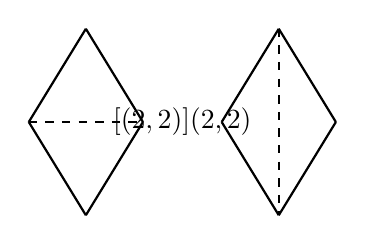
\begin{tikzpicture}
 \def\a{1.45}
 \def\b{0.5}
 \def\trigConst{0.816497}

 %1st Triangle
 \draw[thick, dashed] (-\a-\b,0) -- (-\b, 0);
 \draw[thick] (-\a-\b,0)         -- ({-\b-(0.5*\a)}, {\trigConst * \a});
 \draw[thick] (-\b,0)    -- ({-\b-(0.5*\a)}, {\trigConst * \a});
 \draw[thick] (-\a-\b,0)         -- ({-\b-(0.5*\a)}, {-\trigConst * \a});
 \draw[thick] (-\b,0)            -- ({-\b-(0.5*\a)}, {-\trigConst * \a});


 %2nd Triangle
 \draw[thick, dashed] ({\b+(0.5*\a)}, {\trigConst * \a}) -- ({\b+(0.5*\a)}, {-\trigConst * \a});
 \draw[thick] (\a+\b,0)                                  -- ({\b+(0.5*\a)}, {\trigConst * \a});
 \draw[thick] (\b,0)                                     -- ({\b+(0.5*\a)}, {\trigConst * \a});
 \draw[thick] (\a+\b,0)                                  -- ({\b+(0.5*\a)}, -{\trigConst * \a});
 \draw[thick] (\b,0)                                     -- ({\b+(0.5*\a)}, -{\trigConst * \a});

 %Lines to center

 \node[align=center] at (0,0) {$\xrightleftharpoons[(2,2)]{(2,2)}$};
\end{tikzpicture}
}
    \end{block}
   \end{column}}
  \begin{column}{0.27\textwidth}
   \uncover<7->{\begin{block}{3D}
     \vspace{0pt}
     
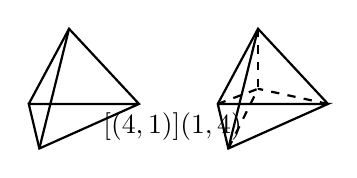
\begin{tikzpicture}[scale=1]
 \def\a{1.40}
 \def\b{0.5}
 \def\trigConst{0.816497}


 \begin{scope} [x     = {(1cm,0)},
   y     = {({0.7cm*cos(135)},{-0.7cm*sin(135)})},
   z     = {(0,1cm)}]

  \path coordinate (T1) at ({-(\b + (0.5*\a))}, {0.3333*\trigConst*\a}, {\trigConst*\a})
  coordinate (A1) at ({-\b},0,0)
  coordinate (B1) at ({-(\a + \b)},0,0)
  coordinate (C1) at ({-(\b + (0.5*\a))},{\trigConst*\a},0);


  \path coordinate (T2) at ({(\b + (0.5*\a))}, {0.3333*\trigConst*\a}, {\trigConst*\a})
  coordinate (A2) at ({\b},0,0)
  coordinate (B2) at ({(\a + \b)},0,0)
  coordinate (C2) at ({(\b + (0.5*\a))},{\trigConst*\a},0)
  coordinate (D2) at ({(\b + (0.5*\a))}, {0.3333*\trigConst*\a}, {0.3333*\trigConst*\a});


  \draw[thick]  (A1)  -- (B1) -- (C1) -- (A1) -- (T1) -- (B1);
  \draw[thick]  (C1) -- (T1);

  \draw[thick]  (A2)  -- (B2) -- (C2) -- (A2) -- (T2) -- (B2);
  \draw[thick]  (C2) -- (T2);

  \draw[thick, dashed] (A2) -- (D2);
  \draw[thick, dashed] (B2) -- (D2);
  \draw[thick, dashed] (C2) -- (D2);
  \draw[thick, dashed] (T2) -- (D2);

  \node[align=center] at ({0.15*\a},{0.5*\trigConst*\a},0) {$\xrightleftharpoons[(4,1)]{(1,4)}$};

 \end{scope}
\end{tikzpicture}
\\
     \vspace{1.0em}
     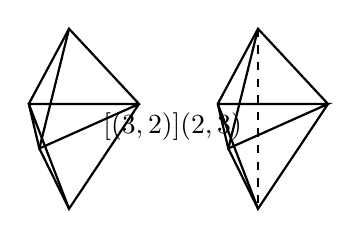
\begin{tikzpicture}[scale=1]
 \def\a{1.40}
 \def\b{0.5}
 \def\trigConst{0.816497}

 \begin{scope} [x     = {(1cm,0)},
   y     = {({0.7cm*cos(135)},{-0.7cm*sin(135)})},
   z     = {(0,1cm)}]


  \path coordinate (T1) at ({-(\b + (0.5*\a))}, {0.3333*\trigConst*\a}, {\trigConst*\a})
  coordinate (A1) at ({-\b},0,0)
  coordinate (B1) at ({-(\a + \b)},0,0)
  coordinate (C1) at ({-(\b + (0.5*\a))},{\trigConst*\a},0)
  coordinate (E1) at ({-(\b + (0.5*\a))}, {0.3333*\trigConst*\a}, {-\trigConst*\a});


  \path coordinate (T2) at ({(\b + (0.5*\a))}, {0.3333*\trigConst*\a}, {\trigConst*\a})
  coordinate (A2) at ({\b},0,0)
  coordinate (B2) at ({(\a + \b)},0,0)
  coordinate (C2) at ({(\b + (0.5*\a))},{\trigConst*\a},0)
  coordinate (D2) at ({(\b + (0.5*\a))}, {0.3333*\trigConst*\a}, {0.3333*\trigConst*\a})
  coordinate (E2) at ({(\b + (0.5*\a))}, {0.3333*\trigConst*\a}, {-\trigConst*\a});


  \draw[thick]  (A1)  -- (B1) -- (C1) -- (A1) -- (T1) -- (B1) -- (E1) -- (A1);
  \draw[thick]  (T1) -- (C1) -- (E1);

  \draw[thick]  (A2)  -- (B2) -- (C2) -- (A2) -- (T2) -- (B2) -- (E2) -- (A2);
  \draw[thick]  (T2) -- (C2) -- (E2);

  \draw[thick, dashed] (T2) -- (E2);


  \node[align=center] at ({0.15*\a},{0.5*\trigConst*\a},0) {$\xrightleftharpoons[(3,2)]{(2,3)}$};

 \end{scope}
\end{tikzpicture}

    \end{block}}
  \end{column}
 \end{columns}
 \uncover<5->{\center{\tiny{As e.g. found in: Banburski, Chen, Freidel, Hnybida \emph{PhysRevD.92.124014}}}}
\end{frame}

\begin{frame}{Problems in four Dimensions}
 \begin{columns}
  \begin{column}{0.48\textwidth}
   \uncover<2->{\begin{block}{Non trivial measure term}
    \vspace{0pt}
    {\tiny{(Laiho, Bassler, Coumbe, Du, Neelakanta \emph{PhysRevD.96.064015})}}
    \begin{align*}
     Z_E = \sum_T \frac{1}{C_T} \left[ \prod_{j=1}^{N_2} \mathcal{O} \left( t_j \right)^\beta \right] \mathrm{e}^{-S_{ER}}
    \end{align*}
    with $\beta \neq 0$.
    \begin{itemize}
     \item $\mathcal{O}(t_j)$ is the \# 4-simplices the triangle $t_j$ belongs to
     \item Discrete limit of $\displaystyle \left[ \mathrm{det} (-g) \right]^{\beta/2}$
     \item Treat $\beta$ as another bare parameter
    \end{itemize}
   \end{block}}
  \end{column}
  \begin{column}{0.48\textwidth}
   \uncover<3->{\begin{block}{Other solutions}
    \vspace{0pt}
    \begin{itemize}
     \item Causal Dynamical Triangulations
           \begin{itemize}
            \item distinguish between space and time links
            \item various causality constraint
           \end{itemize}
    \end{itemize}
   \end{block}}
  \end{column}
 \end{columns}
\end{frame}


\section{Observables}


\begin{frame}{Phase Diagram of EDT and the Continuum limit}
 \begin{figure}
  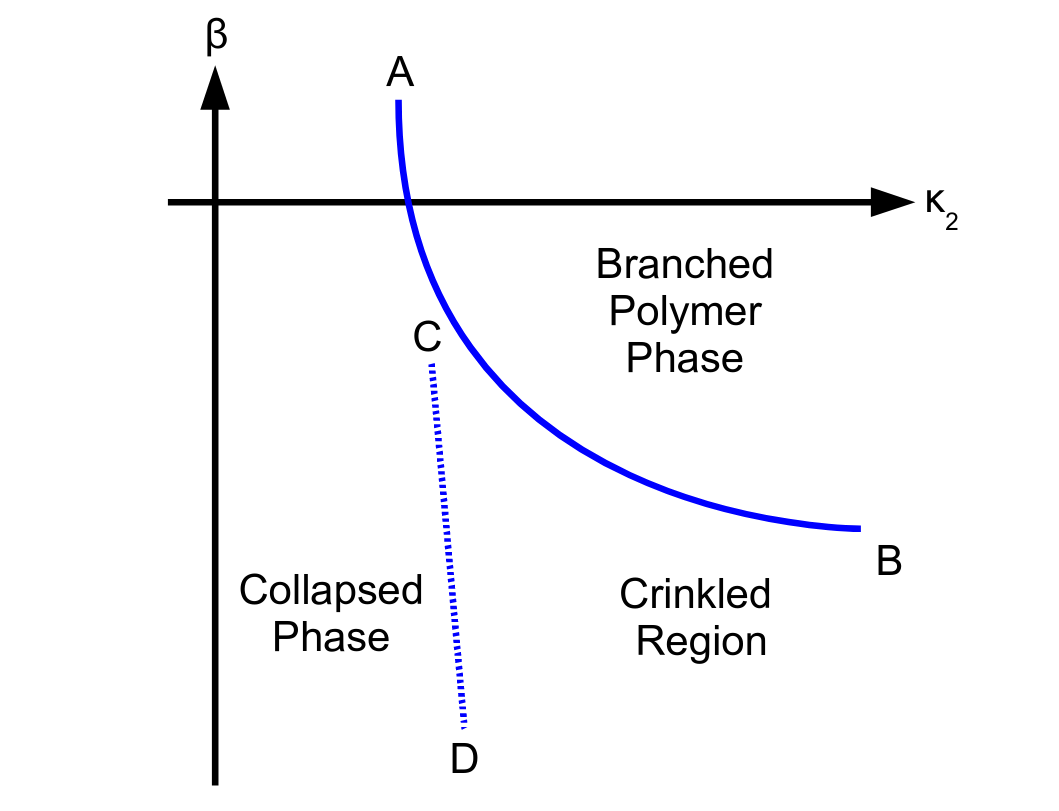
\includegraphics[width=0.6\textwidth]{pics/phase-diagram}
  \caption{SOURCE}
 \end{figure}
\end{frame}

\begin{frame}{Fractal Dimension of the triangulation}
 \begin{columns}
  \begin{column}{0.38\textwidth}
   \begin{figure}
    \centering
    \begin{subfigure}{0.32\textwidth}
     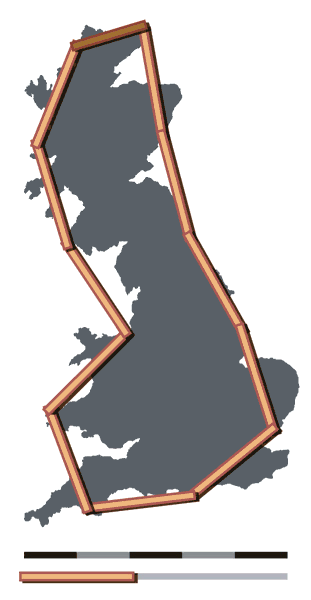
\includegraphics[width=\textwidth]{pics/Britain-fractal-coastline-200km}
     \caption{$\varepsilon=\SI{200}{km}$}
    \end{subfigure}
    \begin{subfigure}{0.32\textwidth}
     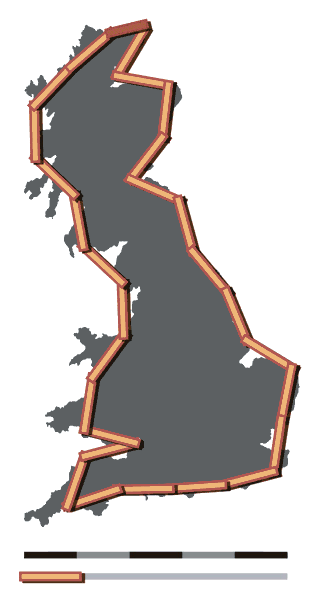
\includegraphics[width=\textwidth]{pics/Britain-fractal-coastline-100km}
     \caption{$\varepsilon=\SI{100}{km}$}
    \end{subfigure}
    \begin{subfigure}{0.32\textwidth}
     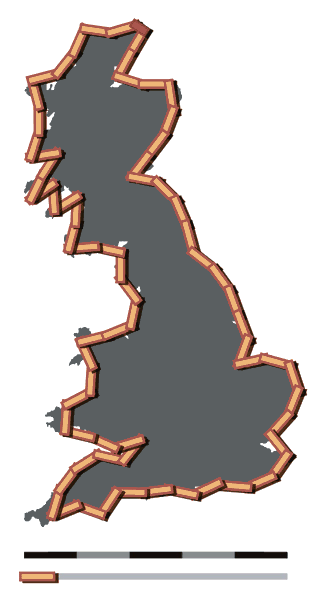
\includegraphics[width=\textwidth]{pics/Britain-fractal-coastline-50km}
     \caption{$\varepsilon=\SI{50}{km}$}
    \end{subfigure}
    \caption{\tiny{Source: \url{https://commons.wikimedia.org/wiki/File:Britain-fractal-coastline-combined.jpg}}}
   \end{figure}
   % Germany: 1.111
   % United Kingdom: 1.215
   % Norway: 1.372
  \end{column}
  \begin{column}{0.58\textwidth}
   \begin{block}{Fractal Dimensions}
    \vspace{0pt}
    \begin{itemize}
     \item Quantifies ''roughness'' of surface
     \item Expect $d=4$ in continuum limit
    \end{itemize}
    \textbf{Box-Counting Dimension}
    \begin{align*}
     d_{\textrm{box}} & = \lim_{\epsilon \rightarrow 0} \frac{\log(N(\varepsilon))}{\log(1/\varepsilon)}
     \intertext{\textbf{Hausdorff Dimension}}
     d_H              & = \lim_{r \rightarrow 0} \frac{\log\left(V(r)\right)}{\log(r)}
    \end{align*}
    where $V(r)$ is the volume of a sphere with radius $r$.
   \end{block}
  \end{column}
 \end{columns}
\end{frame}
\begin{frame}{Fractal Dimensions}
 \begin{columns}[onlytextwidth,t]
  \begin{column}{0.48\textwidth}
   \begin{block}{Measuring the Hausdorff Dimension}

   \end{block}
  \end{column}
  \begin{column}{0.48\textwidth}
   \begin{block}{de Sitter Solution}

   \end{block}
  \end{column}
 \end{columns}
\end{frame}

\begin{frame}
 \begin{columns}[onlytextwidth,t]
  \begin{column}{0.48\textwidth}
   \begin{block}{Spectral Dimensions}
    \begin{align*}
      d_S = \frac{\mathrm{d} \log \left\langle P(\sigma) \right\rangle}{\mathrm{d} \log \sigma}
    \end{align*}
   \end{block}
  \end{column}
  \begin{column}{0.48\textwidth}
   \begin{block}{}

   \end{block}
  \end{column}
 \end{columns}
\end{frame}


\section{Conclusion}


\begin{frame}{Conclusion}
 \begin{columns}
  \begin{column}{0.57\textwidth}
   \begin{block}{Outlook}
    \vspace{0pt}
    \begin{itemize}
     \item Coupling to scalar fields shows Newtonian Binding\\
     {\tiny{Dai, Laiho, Schiffer, Unmuth-Yockey \emph{PhysRevD.103.114511}}}
     \item Extraction of the gravitational constant consistent between pure gravity and scalar fields\\
     {\tiny{Bassler, Laiho, Schiffer, Unmuth-Yockey \emph{PhysRevD.103.114504}}}
     % \item  Kähler Dirac Fermions on EDT\\
     % (Insert Paper Reference)
    \end{itemize}
    %$\rightarrow$ Quantum gravity seems to be asymptotically safe
    %$\rightarrow$ EDT seems to be a promising candidate for quantum gravity
   \end{block}
  \end{column}
  \begin{column}{0.42\textwidth}
   \begin{block}{Sources}
    \begin{itemize}
      \item Laiho, Bassler, Coumbe, Du, Neelakanta \emph{PhysRevD.96.064015}\\
            \emph{Lattice quantum gravity and asymptotic safety}
      \item Cuzinatto, de Melo, Naldoni de Souza \url{arxiv.org/abs/1904.01966}
            \emph{Introduction to Regge Calculus for Gravitation}
    \end{itemize}
   \end{block}
  \end{column}
 \end{columns}
\end{frame}


\begin{frame}
 \resizebox{0.5\textwidth}{!}{The End - Thanks for listening}\\
 \vspace{0.5cm}
 Code can be found at:
\end{frame}

\appendix

\input{sec_bonus}

\end{document}
